%************************************************
\chapter{Introduction}\label{ch:introduction}
%************************************************
\glsresetall % Resets all acronyms to not used

\ac{AnSiAn} is an Android application by the Secure Mobile Network Lab (SEEMOO) at 
Technische Universität Darmstadt. It features a graphical signal analyzer that can be used with common \acp{SDR} like the
HackRF and the RTL-SDR. The project is based on RF~Analyzer, an application by
Dennis Mantz. \ac{AnSiAn} currently extends RF~Analyzer by the following features: 
\begin{itemize}
	\item Time Domain Signal Graph (Waveform)
	\item Morse Decoder
	\item Scanner
	\item Codebase structured according to the \ac{MVC} pattern
\end{itemize}

This lab aims to further extend the feature set of \ac{AnSiAn} while also
making the app more stable and refining existing features. The description of
the project goals are listed in \autoref{sec:project_definition}.


\section{Project Definition\label{sec:project_definition}}

This section defines the features that will be implemented throughout the
project and schedules them into three sprints.

\subsection{Features}

The new features can be divided into mandatory features, that will have high
priority within this project, and optional features, that will be implemented
if time permits. As can be seen in \autoref{sec:time_schedule}, the third
sprint is reserved for either optional features or completing mandatory
features and the documentation.

\subsubsection{Mandatory Features}

The following features are scheduled for implementation during the first and
second sprint:
\begin{itemize}
	\item \ac{RDS} demodulation \\
		If the user selects the existing wide-band \ac{FM} demodulation option,
		the app shall try to detect and demodulate any existing \ac{RDS}
		signal along with the audio demodulation. The extracted information
		shall be displayed on the screen.
	\item \ac{PSK31} demodulation \\
		If the user selects either of the single side band demodulation modes
		(\ac{USB} and \ac{LSB}), he or she shall have the option to enable
		\ac{PSK31} demodulation along with or instead of the audio demodulation.
		The demodulated text string shall appear and scroll through the
		analyzer window.
	\item Extraction of RDS-, Morse- and \ac{PSK31}-data to logfiles \\
		If the user selects to demodulate any digital mode, the demodulated
		text shall be written to a log file specified by the user.
	\item Support for the rad1o badge \\
		The rad1o badge, which is a modified low-cost replica of the HackRF,
		shall be supported as a signal source by AnSiAn.
	\item Transmission support for HackRF and rad1o \\
		If \ac{AnSiAn} is used with an \ac{SDR} capable of transmitting signals,
		it shall offer options to send signals in the following ways:
		\begin{itemize}
			\item Replay I/O samples from a file
			\item Generate and send Morse code from text
			\item FM-modulate and send audio from a file
		\end{itemize}
\end{itemize}

\subsubsection{Optional Features}

The optional features are scheduled in the third and last sprint. However,
they will only be added to the feature set if the last sprint is not needed
in order to compensate for delays on the mandatory features. The optional features are
listed in the order of priority:
\begin{itemize}
	\item Walkie-Talkie Mode \\
		The user shall have the possibility to put AnSiAn into a Walkie-
		Talkie mode. In this mode, the application will demodulate an FM channel
		and the user can quickly switch between demodulation and transmission
		of audio recorded from the internal microphone.
	\item Packet Radio demodulation\\
		A new mode \emph{Packet Radio} shall be added to AnSiAn. Once selected, it shall allow the user
		to tune to a Packet Radio channel and display information about 
		demodulated packets on the screen. If time permits, it might even
		be possible to implement a transmission feature for Packet Radio.
\end{itemize}


\subsection{Time Schedule}
\label{sec:time_schedule}

The project will have two developers, Dennis Mantz and Max Engelhardt,
working in three sprints. There are three milestones corresponding to
the sprints, labeled Alpha, Beta and Final Version. They each add an independent
and self-contained set of features to the application:

\begin{itemize}
	\item Software Design (due 12.05.)
	\item Sprint 1: Alpha Version (due 09.06.)
	\begin{itemize}
		\item \ac{RDS} demodulation
		\item \ac{PSK31} demodulation
		\item Extraction of \ac{RDS}-, Morse- and \ac{PSK31}-data to logfiles
	\end{itemize}
	\item Sprint 2: Beta Version (due 21.07.)
	\begin{itemize}
		\item Support for the rad1o badge
		\item Transmission support for HackRF and rad1o
		\begin{itemize}
			\item Replay I/O samples from a file
			\item Generate and send Morse code from text
			\item FM-modulate and send audio from a file
		\end{itemize}
	\end{itemize}
	\item Sprint 3: Final Version (due 25.08.)
	\begin{itemize}
		\item Complete leftovers from previous sprints
		\item Walkie-Talkie Mode (optional)
		\item Packet Radio demodulation (optional)
	\end{itemize}
\end{itemize}

\section{Software Design}

The software design for each sprint is done ahead of the respective sprint.
This procedure goes along well with the Agile Manifesto which
encourages the design of a complex system in small incremental parts.

\subsection{Sprint 1: PSK31 and RDS demodulation}

The existing architecture of \ac{AnSiAn} features individual threads for scheduling, 
downsampling, demodulation and audio output. The \texttt{De\-mo\-du\-la\-tor} thread demodulates 
quadrature samples by calling the \texttt{demodulate()} method on an instance of
\texttt{Demodulation}. \texttt{Demodulation} is an abstract class that is implemented by concrete 
demodulation methods such as \texttt{AM}, \texttt{FM} and \texttt{Morse}. 

\ac{AnSiAn} utilizes the EventBus library in order to pass demodulated morse text
to the \ac{GUI}. Demodulated audio data is passed to the
\texttt{AudioSink} thread by enqueueing it into its input queue.
This mechanism is explained in more detail in \autoref{sec:cleanup.mem}.


In order to extend \ac{AnSiAn} with demodulation functionality for \ac{PSK31} and \ac{RDS}, 
the existing architecture needs to be extended. The extended architecture is
depicted in \autoref{fig:demod_text_eventbus} and explained in the following.

 \begin{figure}
	\centering
	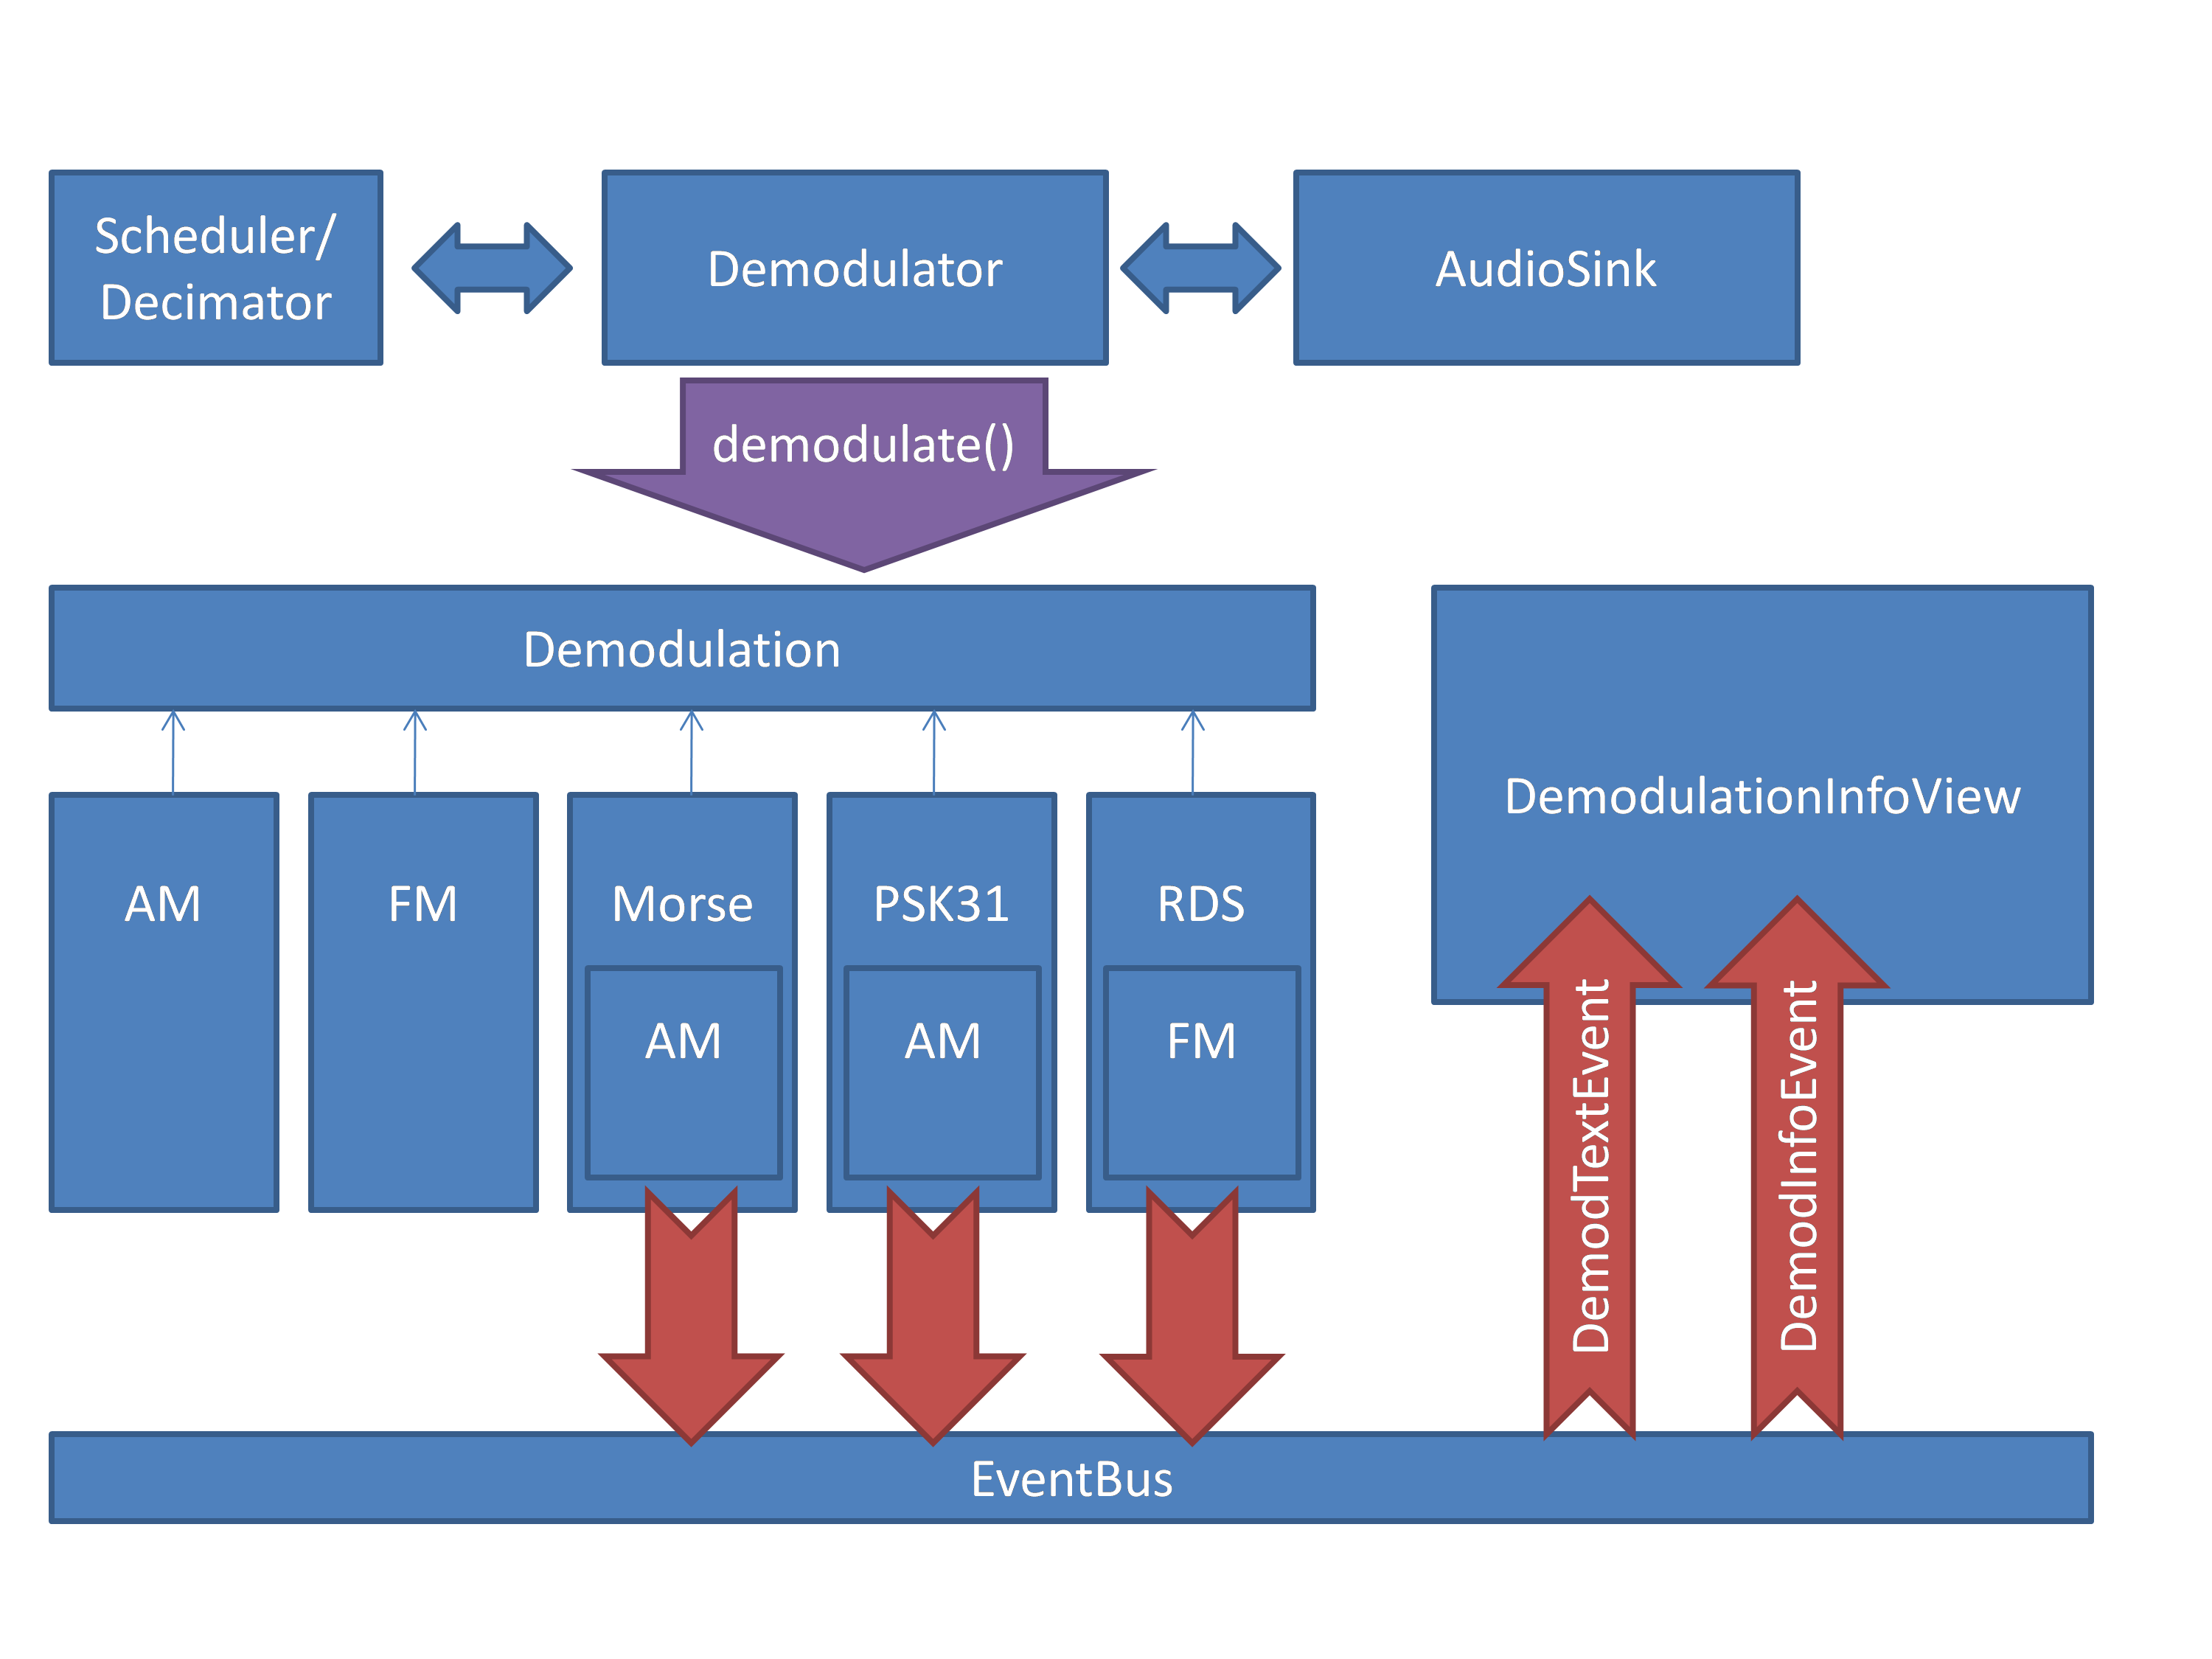
\includegraphics[width=1\linewidth]{gfx/demod_text_eventbus.png}
	\caption{Architecture of the extended demodulation logic and communication with the GUI}
	\label{fig:demod_text_eventbus}
\end{figure}

Two new classes \texttt{PSK31} and \texttt{RDS}, that inherit from
\texttt{Demodulation}, need to be implemented to represent the new demodulation 
mechanisms.

As \ac{PSK31} demodulation works on the envelope of the received signal
and \ac{AM} demodulation essentially performs envelope detection, \texttt{PSK31}
uses an instance of \texttt{AM} for envelope detection.

\ac{RDS} transmits metadata for \ac{FM} radio channels. It is therefore desirable for the 
\ac{RDS} demodulaton mode to not only display this metadata, but to also play the 
\ac{FM}-modulated audio at the same time. The \texttt{RDS} class uses an
instance of \texttt{FM} for this purpose.

Like the existing architecture, the new architecture will use the EventBus
library to pass the demodulated text to the \ac{GUI}. The existing View
\texttt{MorseReceiveView} is refactored into a universal
\texttt{De\-mo\-du\-la\-tion\-In\-fo\-View} that displays the text output of any selected 
demodulator. Demodulators pass \texttt{DemodTextEvent}s and 
\texttt{DemodInfoEvent}s via the EventBus to the \texttt{De\-mo\-du\-la\-tion\-In\-fo\-View}, 
which contain demodulated text and further information (e.g. baud rates or raw 
dits and dahs) and are displayed in separate lines.



\section{Cleanup Tasks\label{sec:cleanup}}

\subsection{Memory Optimizations\label{sec:cleanup.mem}}


%%*****************************************
%\chapter{Related Work}\label{ch:relatedwork}
%%*****************************************
%\glsresetall % Resets all acronyms to not used
%
%\lipsum[4]
